\documentclass[letter]{article}
\renewcommand{\baselinestretch}{1.25}

\usepackage[margin=1in]{geometry}
\usepackage{physics}
\usepackage{amsmath}
\usepackage{graphicx}
\usepackage{hyperref}


% MATLAB Formating Code
\usepackage[numbered,framed]{matlab-prettifier}
\lstset{style=Matlab-editor,columns=fullflexible}
\renewcommand{\lstlistingname}{Script}
\newcommand{\scriptname}{\lstlistingname}



% Document Specific
\newcommand{\sat}{\text{sat}}


\allowdisplaybreaks

%opening
\title{MECH 6313 - Homework 5}
\author{Jonas Wagner}
\date{2021, April 14}

\begin{document}

\maketitle

\tableofcontents

\newpage

\section{Problem 1}
The standard mass-spring-damper system described by
\begin{equation}
	m \ddot{y} + \beta \dot{y} + k y = u
\end{equation}

\subsection{Part a}
\textbf{Problem:}
Design a gradient algorithm to estimate the unknown parameters $m$, $\beta$, and $k$ from known inputs and outputs $u(t)$ and $y(t)$.\\

\noindent
\textbf{Solution:}
The system identification problem can be reformatted for a recursive estimator for constant parameters as follows:\\

First he spring-mass-damper dynamics can be rewritten in the following form:
\begin{align}
	\ddot{y} &= - \frac{\beta}{m} \dot{y} - \frac{k}{m} y + \frac{1}{m} u\\
	s^2 Y &= - \frac{\beta}{m} s Y - \frac{k}{m} Y + \frac{1}{m} U
	\intertext{Letting $\Lambda(s) = s^2 + \lambda_1 s + \lambda_0$ to represent the charectoristic polynomial of a 2nd-order filter,}
	\frac{s^2 Y}{\Lambda(s)} &= \frac{- \frac{\beta}{m} s Y - \frac{k}{m} Y + \frac{1}{m} U}{\Lambda(s)}
\end{align}


\begin{align}
	Y(s) &= \qty(\frac{1}{m}) \frac{1}{\Lambda(s)} U - \qty(\frac{\beta}{m} - \lambda_1) \frac{s}{\Lambda(s)} Y - \qty(\frac{k}{m} - \lambda_0) \frac{1}{\Lambda(s)} Y
\end{align}

Let
\begin{equation}
	\theta = \mqty[\frac{1}{m}\\ \frac{\beta}{m} - \lambda_1 \\ \frac{k}{m} - \lambda_0] = \mqty[b_1\\ \bar{a}_1 \\ \bar{a}_0] = \mqty[\theta_1 \\ \theta_2 \\ \theta_3]
\end{equation}

Known measured and imputed quantities can then be defined as
\begin{equation}
	\Psi(s) = \mqty[\psi_1\\ \psi_2 \\ \psi_3]
	= \mqty[\cfrac{1}{\Lambda(s)} U \\ \cfrac{-s}{\Lambda(s)} Y\\ \cfrac{-1}{\Lambda(s)} Y]
\end{equation}

which can be used alongside the unknown parameters to define the following standard form parameter estimation problem:
\begin{equation}
	Y(s) = \Psi(s)^T \Theta
\end{equation}

This can then be further developed to define a gradient-based parameter estimator.\\

First, let $\hat{\Theta}$ be defined as the estimate of the parameters $\Theta$ and the estimation error, $\tilde{\Theta}$ of the parameter be defined as $$\tilde{\Theta}(t) = \Theta - \hat{\Theta}(t)$$ and the convergence dynamics should be defined as $$\dot{\tilde{\Theta}}(t) = - \dot{\hat{\Theta}}(t)$$

Subsequently the output error is can be defined in terms of the parameter error by the following:
\begin{align}
	e(t)
	&= y(t) - \hat{y}(t)\\
	&= \Psi^T(t) \Theta - \Psi^T(t) \hat{\Theta}(t)\\
	&= \Psi^T(t) \qty[\Theta - \hat{\Theta}(t)]\\
	&= \Psi^T(t) \tilde{\Theta}(t)
\end{align}

A simple gradient decent algorithm can then be defined by:
\begin{align}
	\frac{1}{2} e^2(t)
	&= \frac{1}{2} e^T(t) e(t)\\
	&= \frac{1}{2} \tilde{\Theta}^T(t) \Psi(t) \Psi^T(t) \tilde{\Theta}
\end{align}
and since
\begin{equation}
	\dot{\tilde{\Theta}} = - \grad_{\tilde{\Theta}} \qty[\frac{1}{2} e^2(t)]\\
\end{equation}
an LTV system can be defined as
\begin{align}
	\dot{\tilde{\Theta}} &= -\Psi(t) \Psi^T(t) \tilde{\Theta}
	\intertext{or equivelently, since $e(t) = \Psi^T(t) \tilde{\Theta}(t)$}
	\dot{\tilde{\Theta}} &= -\Psi(t) \Psi^T(t) e(t)
\end{align}

This algorithm can then be implemented for this specific system by defining the estimator dynamic matrice as:
\begin{equation}
	\begin{aligned}
		A &= \Psi(t) \Psi^T(t)\\
		B &= - \Psi(t)
	\end{aligned}
\end{equation}

\newpage
\subsubsection{Part b}
\textbf{Problem:}
Simulate the algorithm for $m = 20$, $\beta = 0.1$, and $k = 5$ for different choices of $u(t)$ and resulting parameter convergence properties.\\

\noindent
\textbf{Solution:}
This was simulated in MATLAB using Simulink. The code can be found in \appendixname \ref{apx:matlab}. The simulink model can be seen in \figurename \ \ref{fig:pblm1b_model}.

\begin{figure}[h]
	\centering
	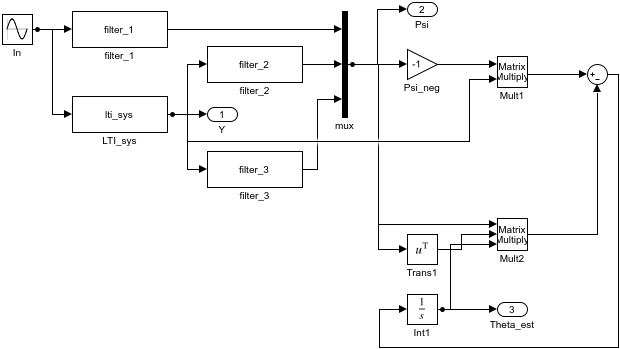
\includegraphics[width=\linewidth]{fig/sim_model_pblm1b}
	\caption{Simulink Model used to simulate the parameter estimation}
	\label{fig:pblm1b_model}
\end{figure}

\newpage
The simulation results can be seen in \figurename \ \ref{fig:pblm1b_results}

\begin{figure}[h]
	\centering
	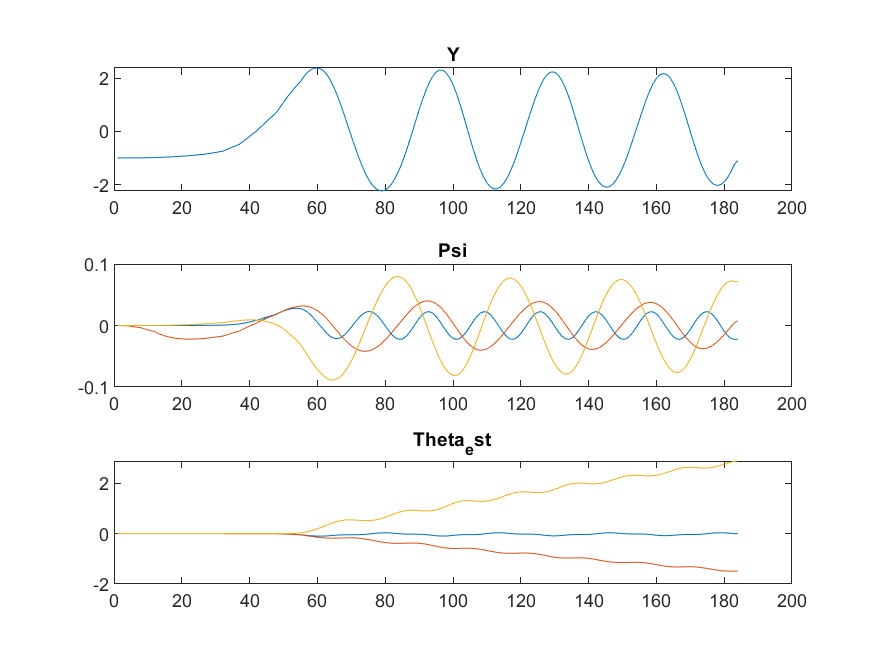
\includegraphics[width=\linewidth]{fig/pblm1b_results}
	\caption{Simulink Results}
	\label{fig:pblm1b_results}
\end{figure}

\newpage
\section{Problem 2}
Considering the reference model
\begin{equation}
	\dot{y}_m = -a y_m + r(t), \ a>0
\end{equation}
and the plant given as
\begin{equation}
	\dot{y} = a^*y + b^* u, \ b^* \neq 0
\end{equation}

\subsection{Part a}
\textbf{Problem:}
Show that a controller of form $$u = \theta_1 y + \theta_2 r(t)$$ with gains $\theta^*_1$ and $\theta^*_2$ stabilizes the tracking error $e:= y-y_m$ asymptotically to zero.\\

\noindent
\textbf{Solution:}
A method to achieve the calculate the tracking error is to implement a Model Reference Adaptive Controller (MRAC) that will change the dynamics of the plant into the reference model. In an ideal case, the parameters $a$ and $b$ will be known and a control law, $u = \theta_1^* y + \theta_2^* r(t)$, can be defined directly as follows:
\begin{align}
	-a y_m + r(t) = \dot{y}_m = \dot{y}
	&= a^* y + b^* (\theta_1^* y + \theta_2^* r(t))\\
	-a y_m + r(t)
	&= (a^* + b^* \theta_1) y + b^* \theta_2 r(t)
\end{align}
Clearly they dynamics are therefore equivalent if the following are true:
\begin{align}
	- a &= (a^* + b^* \theta_1^*)\\
	1	&= b^* \theta_2^*
\end{align}
Thus these dynamics would be equivalent dynamics for gains defined as:
\begin{align}
	\theta_1^* &= \frac{-(a + a^*)}{b^*}\\
	\theta_2^* &= \frac{1}{b^*}
\end{align}
The error dynamics for $$e(t) = y - y_m$$ can be defined as
\begin{align}
	\dot{e}(t) &= \dv{t} (y - y_m)\\
	&= (a^* + b^* \theta_1^*) y + b^* \theta_2^* r(t) - ( -a y_m + r(t))\\
	&= (a^* + b^* \frac{-(a + a^*)}{b^*}) y + b^* \frac{1}{b^*} r(t) - ( -a y_m + r(t))\\
	&= -(a^* - a^* + a)y + r(t) - (-a y_m + r(t))\\
	&= -a y - a (-y_m) = -a (y-y_m)\\
	\dot{e} &= - a e\label{eq:dot_e}
\end{align}
which for $a>0$ is clearly GAS.


\subsection{Part b}
\textbf{Problem:}
Suppose $a^*$ and $b*$ are unknown but the sign of $b^*$ is known. Show that the adaptive implementation of the controller can achieve tracking when the gains are updated according to the following rule:
\begin{equation} \label{eq:dot_theta}
	\begin{aligned}
		& \dot{\theta}_1 = - \text{sign}(b^*) \gamma_1 y e\\
		& \dot{\theta}_2 = - \text{sign}(b^*) \gamma_2 r e
	\end{aligned}
\end{equation}
with $\gamma_1, \gamma_2 > 0$.\\

\noindent
\textbf{Solution:}
Effective tracking occurs when the error, $e = y - y_m$, asymptotically decays to zero. For the MRAC with control law defined as $$u=\theta_1 y + \theta_2 r$$ the asymptotic stability can be demonstrated as follows:
Let
\begin{align}
	\tilde{\theta}_1 = \theta_1 - \theta_1^*\\
	\tilde{\theta}_2 = \theta_2 - \theta_2^*
\end{align}
then the following equivalent gains
\begin{align}
	\theta_1 = \theta_1^* + \tilde{\theta}_1\\
	\theta_2 = \theta_2^* + \tilde{\theta}_2
\end{align}
can be substituted into the error dynamics
\begin{align}
	\dot{e}(t) &= \dv{t} (y - y_m)\\
	&= (a^* + b^* \theta_1) y + b^* \theta_2 r(t) - ( -a y_m + r(t))\\
	&= (a^* + b^* (\theta_1^* + \tilde{\theta}_1)) y + b^* (\theta_2^* + \tilde{\theta}_2) r(t) - ( -a y_m + r(t))\\
	&=(a^* + b^* \theta_1^*) y + b^* \theta_2^* r(t) - ( -a y_m + r(t)) + b^* \tilde{\theta}_1 y + b^* \tilde{\theta}_2 r(t)\\
	&= (a^* + b^* \frac{-(a + a^*)}{b^*}) y + b^* \frac{1}{b^*} r(t) - ( -a y_m + r(t)) b^* \tilde{\theta}_1 y + b^* \tilde{\theta}_2 r(t)\\
	&= -(a^* - a^* + a)y + r(t) - (-a y_m + r(t)) + b^* \tilde{\theta}_1 y + b^* \tilde{\theta}_2 r(t)\\
	&= -a(y-y_m) + b^* (\tilde{\theta}_1 y + \tilde{\theta}_2 r(t))\\
	&= -(a)e(t) + b^* (\tilde{\theta}_1 y + \tilde{\theta}_2 r(t)) \label{eq:dot_e_with_theta}
\end{align}
From this it is clear that the error dynamics are the same as the ideal plus the additional terms associated with the gain errors.

Therefore effective tracking can be achieved if the combined system defined as follows by combining \eqref{eq:dot_e_with_theta} with the time derivatives of gain errors (equivalent to \eqref{eq:dot_theta}):
\begin{equation}\label{eq:addaptive_error_dynamics}
	\begin{aligned}
		\dot{e}(t) &= -(a)e + b^* (\tilde{\theta}_1 y + \tilde{\theta}_2 r(t))\\
		\dot{\tilde{\theta}}_1 &= - \tilde{\gamma}_1 \ y \ e\\
		\dot{\tilde{\theta}}_2 &= - \tilde{\gamma}_2 \ r \ e
	\end{aligned}
\end{equation}
where $\text{sign}(\tilde{\gamma}_i) = \text{sign}(b^*)$ and $\abs{\tilde{\gamma}_i} = \abs{\gamma_i}$ for $i=1,2$.

\subsubsection{Error Dynamics Origin Stability}
Upon analysis of \eqref{eq:addaptive_error_dynamics}, it is clear that there is an equilibrium point when $$e = \dot{\tilde{\theta}}_1 = \dot{\tilde{\theta}}_2 = 0$$ and since an effective tracker exists at that equilibrium point, if the error dynamics are GAS about that point then it is an effective tracker.

The linearized system matrices about the equivalent origin is given as
\begin{equation}
	\begin{aligned}
		A &= \eval{\mqty[-a &b^* y &b^* r\\
				  - \tilde{\gamma}_1 \ y & 0 &0\\
				  - \tilde{\gamma}_2 \ r & 0 & 0]
			  	  }_{y=r=0}
		   = \mqty[-a & &\\&0&\\&&0]\\
%		B &= \eval{\mqty[ b^* \tilde{\theta}_1 & b^* \tilde{\theta}_2\\
%				  -\tilde{\gamma}_1 e & 0\\ 
%				  -\tilde{\gamma}_2 e & 0]}_{\tilde{\theta}_1 = \tilde{\theta}_2= y = r = 0}
%		   = \vb{0}_{3\cross2}
	\end{aligned}
\end{equation}
with $x = \mqty[e\\ \tilde{\theta}_1 \\ \tilde{\theta}_2]$ and time-varying parameters $y$ and $r(t)$.

It is clear the linearzed system is at least marginally zero so any tracking errors caused will at least be bounded locally. It is also clear that if the dynamic gain component is ignored, the error will asymptotically approach zero as demonstrated by \eqref{eq:dot_e}.This isn't enough to demonstrate GAS though.


\subsubsection{Error Lyapnov Equation}
Using a lyapnov function $$x^T P x$$ for $P = \frac{1}{2} I_3$ the error dynamics at the origin can be better analyzed.

In this case the a similarly structured time varying system system will be defined as
\begin{equation}
	\begin{aligned}
		\dot{e} 
		&= -a e + b y(t) \theta_1 + b r(t) \theta_2\\
		\dot{\theta_1}	&= - c_1 y(t) e\\
		\dot{\theta_2}	&= - c_2 r(t) e
	\end{aligned}
\end{equation}
with time varying parameters being the signals $y(t)$ and $r(t)$, along with scaler constants $a, b, c_1, c_2$.

For a state vector $x = \mqty[e \\ \theta_1 \\ \theta_2]$, the LTV state-space dynamics can be defined by:
\begin{equation}
	A = \mqty[-a & b y(t) & b r(t)\\
			  -c_1 y(t) & 0 &0\\
			  -c_2 r(t) & 0 &0]
\end{equation}

The stability of these dynamics can be tested for the same marginal stability as shown previously by applying Lyopnov methods with $P=\frac{1}{2} I_3$.

\begin{align}
	V(e, \theta_1, \theta_2) = x^T P x
	&= \frac{1}{2} e^2 + \frac{1}{2} \theta_1^2 + \frac{1}{2} \theta_2^2\\
	\dot{V}(e, \theta_1, \theta_2) = 2 P x^T \dot{x}
	&= e \dot{e} + \theta_1 \dot{\theta_1} + \theta_2 \dot{\theta_2}\\
\end{align}
\begin{align}
	\dot{V} = x^T (2 \qty(\frac{1}{2}) I_3)\dot{x}
	&= e \qty(-a e + b y(t) \theta_1 + b r(t) \theta_2)
	+ \theta_1 (- c_1 y(t) e)
	+ \theta_2 (- c_2 r(t) e)\\
	&= -a e^2 + (b-c_1) (y(t)) (\theta_1 e) + (b - c_1) (r(t)) (\theta_2 e)\\
	&= - x^T \mqty[\dmat{a,0,0}] x + (b-c_1) (y(t)) (\theta_1 e) + (b - c_1) (r(t)) (\theta_2 e)\label{eq:v_dot_result}
\end{align}
from this the observation, once again, of marginal stability (at the origin) is obvious. For design of the tracking error itself, the $Q = \mqty[\dmat{a,0,0}]$ matrix can be used to generate an observation matrix $C$.\\

Since $\dot{V} = -x^T Q x = -x^T C^T C x$, $C$ can be found as
\begin{align}
	Q &= C^T C\\
	\mqty[\dmat{a,0,0}] &= \mqty[\sqrt{a}\\0\\0] \mqty[\sqrt{a}&0&0]
\end{align}
therefore,
\begin{equation}
	C = \mqty[\sqrt{a} & 0 & 0]
\end{equation}


\subsubsection{Universal Observability of (A+LC,C)}
Uniform observability (UO) of the pair $$\qty(A(t), C(t))$$ can then be assured by first confirming UO of $$A(t) + L(t) C(t), C(t)$$ by defining
\begin{equation}
	L(t) = \mqty[\sqrt{a}\\
				 \qty(\cfrac{1}{\sqrt{a}})y(t)\\
				 \qty(\cfrac{1}{\sqrt{a}})r(t)]
\end{equation}
and then calculating
\begin{align}
	A(t) + L(t) C(t)
	&= \mqty[-a & b y(t) & b r(t)\\
			-c_1 y(t) & 0 &0\\
			-c_2 r(t) & 0 &0]
	+ \mqty[\sqrt{a}\\
			\qty(\cfrac{c_1}{\sqrt{a}})y(t)\\
			\qty(\cfrac{c_2}{\sqrt{a}})r(t)]
	  \mqty[\sqrt{a} & 0 & 0]\\
	&= \mqty[-a & b y(t) & b r(t)\\
			-c_1 y(t) & 0 &0\\
			-c_2 r(t) & 0 &0]
	+  \mqty[a & 0 & 0\\
			c_1 y(t) & 0 &0\\
			c_2 r(t) & 0 &0]
\end{align}
\begin{align}
	A(t) + L(t) C(t)
	&= \mqty[0 & b y(t) & b r(t)\\
			0 & 0 &0\\
			0 & 0 &0]
\end{align}

The pair $\qty(A(t) + L(t) C(t), C(t))$ is clearly observable as the output of a system governed by these dynamics would output
\begin{equation}
	y = \sqrt{a} \ b \ (\theta_1 y(t) + \theta_2 r(t))
\end{equation}
which, assuming $y(t)$ and $r(t)$ is known, can be used to calculate all of the states.

This uniform stability can be confirmed for the pair $\qty(A(t) + L(t) C(t), C(t))$ by recognizing that UO for the system:
\begin{equation}
	\begin{aligned}
		\dot{x}
		&= (A(t) + L(t) C(t))
		= \mqty[0 & b y(t) & b r(t)\\
				0 & 0 &0\\
				0 & 0 &0] x\\
		\hat{y}
		&= C x = \mqty[\sqrt{a} & 0 & 0] x
	\end{aligned}
\end{equation}
is the same as stating UO of the system:
\begin{equation}
	\begin{aligned}
		\dot{x}_{2,3}
		&= \vb{0}_2 x\\
		\hat{y}_{2,3}
		&= \sqrt{a} b \mqty[y(t) & r(t)] x_{2,3}
	\end{aligned}
\end{equation}
and this single $C$ matrix can be used to prove UO.\\

UO (and UAS) if $\exists \delta, \ \alpha > 0$ s.t.
\begin{align}
	\int_{t_0}^{t_0+\delta} C C^T \dd{t}
	&\geq \alpha \vb{I}_2 \ \forall t_0\\
	\int_{t_0}^{t_0+\delta} (\sqrt{a} b)^2 \mqty[y(t) & r(t)] \mqty[y(t) \\ r(t)]  \dd{t}
	&\geq \alpha \vb{I}_2 \ \forall t_0\\
	a b^2 \int_{t_0}^{t_0+\delta} (y(t))^2 + (r(t))^2 \dd{t}
	&\geq \alpha \vb{I}_2 \ \forall t_0\label{eq:obsv_gram}
\end{align}
which is clearly true for $y(t)$ and $r(t)$ that are persistently excited.

From this it can be concluded that the system is UAS. This can then be applied to to the original system noting that $c_i = \text{sign}(b^*) \gamma_i \ \forall i = 1,2$.


\newpage
\subsection{Part c}
\textbf{Problem:}
Provide conditions that also guarantee that $\theta_1(t) \to \theta_1^*$ and $\theta_2(t) \to \theta_2^*$ as $t\to\infty$.\\

\noindent
\textbf{Solution:}

From the definition of the ideal control, $u = \theta_1^* y + \theta_2^* r$, it is known that if $\theta_1(t) \to \theta_1^*$ and $\theta_2(t) \to \theta_2^*$ then the MRAC will effectively transform the plant dynamics to that of the reference model.

For the dynamics of the gains, it can be seen from \eqref{eq:v_dot_result} that for GAS, the following must be true:
\begin{align}
	\dot{V} &= -a e^2 + (b-\text{sign}(b^*) \gamma_1) (y(t)) (\tilde{\theta}_1 e) + (b - \text{sign}(b^*) \gamma_2) (r(t)) (\tilde{\theta}_2 e) \prec 0
\end{align}
Originally the terms that were not obviously $\preceq 0$ were ignored as they will at a minimum remain bounded. In order to also insure $\theta_1(t) \to \theta_1^*$ and $\theta_2(t) \to \theta_2^*$, the two other terms must be $\prec 0$.

From \eqref{eq:obsv_gram} it is known that the system is UO and therefore UAS regardless of the system parameters or tun-able $\gamma$ constants, but this is guaranteed when it is known $y(t)$ and $r(t)$ are persistently excited.


\newpage
\section{Problem 3}
A simplified model of an axial compressor, used in jet engine control studies, is given by the following second order system:
\begin{equation}
	\begin{aligned}
		&\dot{\phi} = - \frac{3}{2} \phi^2 - \frac{1}{2} \phi^3 - \psi\\
		&\dot{\psi} = \frac{1}{\beta^2}(\phi + 1 - u)
	\end{aligned}
\end{equation}
This model captures the main surge instability between the mass flow and the pressure rise. Here, $\phi$ and $\psi$ are deviations of the mass flow and the pressure rise from their set points, the control input $u$ is the flow through the throttle, and $\beta$ is a positive constant.

\subsection{Part a}
\textbf{Problem:}
Use backstopping to obtain a control law to stabilize the origin.\\

\noindent
\textbf{Solution:}
This problem can be written in a more standard form of
\begin{align}\label{eq:backstep_original}
	\dot{x_1} &= f(x_1) + g(x_1) x_2\nonumber\\
	\dot{x_2} &= f_a(x_1,x_2) + g_a(x_1,x_2) u
\end{align}
where
\begin{align}
	f(x_1) &= -\frac{3}{2} x_1^2 - \frac{1}{2} x_1^3\\
	&g(x_1) = -1\nonumber \\
	f_a(x_1,x_2) &= \frac{1}{\beta^2} \qty(x_1 + 1)\\
	&g_a(x_1,x_2) = -1\nonumber
\end{align}
and the state variables and inputs are defined such that $x_1 = \phi$, $x_2 = \psi$, and $u = u$.

First looking at the $x_1$ state equation independently and considering the $x_2$ state as an input, $z_1$, a proposed lyapnov equation $$V_1(x_1) = \frac{1}{2} x_1^2$$ can be used to develop a virtual control signal $\alpha(x_1)$.
\begin{align}
	\dot{V}(x_1)
	&= \dv{V}{x_1} \dot{x_1}\\
	&= x_1 \qty(f(x_1) + g(x_1) \alpha(x_1))\\
	&= x_1 \qty(-\frac{3}{2} x_1^2 - \frac{1}{2} x_1^3 - \alpha(x_1))\\
	&= -\frac{3}{2} x_1^3 - \frac{1}{2} x_1^4 - x_1 \alpha(x_1)
\end{align}
Since $-\frac{3}{2} x_1^3$ is not negative definite, $\alpha(x_1)$ can be defined as $$\alpha(x_1) = -\frac{3}{2} x_1^2 + K_1 x_1, \ K_1 > 0$$ and substituted in to cancel it out and add an additional asymptotically decreasing term
\begin{align}
	\dot{V}(x_1)
	&= -\frac{3}{2} x_1^3 - \frac{1}{2} x_1^4 - x_1 \qty(-\frac{3}{2} x_1^3 + K x_1)\\
	&= -\frac{3}{2} x_1^3 - \frac{1}{2} x_1^4  + \frac{3}{2} x_1^3 - K_1 x_1^2, \ K_1 >0\\
	&= -\frac{1}{2} x_1^4 - K_1 x_1^2 \leq -W_1(x_1) < 0, \ K_1 > 0
\end{align}
Clearly this is negative definite, so the virtual control signal of $\alpha(x_1) = -\frac{3}{2} x_1^2 + K_1 x_1$ is acceptable.\\

Next, define the additional state equation
\begin{align}
	z_2
	&= x_2 - \alpha(x_1)\\
	\dot{z_2}
	&= \dot{x_2} - \dot{\alpha}\\
%	&= f_a(x_1,x_2) + g(x_1,x_2) u - \dv{\alpha}{x_1} \dot{x_1}\\
%	&= \frac{1}{\beta^2} \qty(x_1 + 1 - u) - \dv{\alpha}{x_1} \qty[f(x_1) + g(x_1)z]\\
%	&= \frac{1}{\beta^2} \qty(x_1 + 1 - u) u - \dv{\alpha}{x_1} \qty[-\frac{3}{2} x_1^2 - \frac{1}{2} x_1^3 - x_2]
%	\intertext{Next, $z_2 + \alpha(x_1)$ can be substituted into $x_2$ after defining $z_2 = x_2 - \alpha(x_1)$}
%	&= \frac{1}{\beta^2} \qty(x_1 + 1 - u) - \dv{\alpha}{x_1} \qty[-\frac{3}{2} x_1^2 - \frac{1}{2} x_1^3 - z_2 - \alpha(x_1)]
\end{align}

Next, an augmented Lyapnov function:
\begin{align}
	V_a(x_1,z_2)
	&= V_1 (x_1) + \frac{1}{2} z_2^2\\
	&= \frac{1}{2} x_1^2 + \frac{1}{2} z_2^2
\end{align}
stability can then be guaranteed as follows:
\begin{align}
	\dot{V}_a(x_1,z_2)
	&= \dot{V}_1 + z_2 \dot{z_2}\\
	&= \dot{V}_1 + z_2 (\dot{x_2} - \dot{\alpha})\\
	&= \dot{V}_1 + z_2 ((\frac{1}{\beta^2} \qty(x_1 + 1 - u)) - \dot{\alpha})
\end{align}
since $\dot{V}_1 \leq -W_1(x_1)$ this component is not problematic. Thus, setting
$$u = -x_1 - \dot{\alpha} + \beta^2 k_2 z_2, \ k_2 > 0$$
can be used to generate the following
\begin{align}
	\dot{V}_a &= \dot{v_1} - z_2(-k_2 z_2)\\
	&= - W_1(x_1) - k_2 z_2^2 < 0
\end{align}
Which means a control signal of
\begin{equation}
	u =  -x_1 - \dot{\alpha} + \beta^2 k_2 \qty(x_2 - \alpha(x_1)), \ k_2 > 0
\end{equation}
can be implemented in a static nonlinear controller to ensure GAS at the origin.

\newpage
\subsubsection{Part b}
\textbf{Problem:}
Use Sontag's Formula and the Control Lyapunov Function obtained previously to obtain an alternative control law.\\

\noindent
\textbf{Solution:}
The Control Lyapunov Function (CLF) that comes from the previous problem was calculated as
\begin{align}
	\dv{V}{x} f(x) + \dv{V}{x} g(x) \alpha(x) &< 0\\
	(-\frac{3}{2} x_1^3 - \frac{1}{2} x_1^4) + (- x_1 \alpha(x_1)) &< 0
\end{align}
since $$\dv{V}{x} f(x) + \dv{V}{x} g(x) \alpha(x) = L_f V(x) + L_g V(x) \alpha < 0$$
the CLF components are given as
\begin{align}
	L_f V(x) &= -\frac{3}{2} x_1^3 - \frac{1}{2} x_1^4\\
	L_g V(x) &= - x_1
\end{align}

This can then be entered into Sontag's Formula to attain a virtual control function of
\begin{align}
	\alpha(x) 
	&=
	\begin{cases}
		0,	& L_g V(x) = 0\\
		-\cfrac{L_f V(x) + \sqrt{(L_f V(x))^2 + (L_g V(x))^2}}{L_g V(x)}, &\text{otherwise}
	\end{cases}\\
	&=
	\begin{cases}
		0,	& - x_1 = 0\\
		-\cfrac{(-\frac{3}{2} x_1^3 - \frac{1}{2} x_1^4) + \sqrt{(-\frac{3}{2} x_1^3 - \frac{1}{2} x_1^4)^2 + (- x_1)^2}}{- x_1}, &\text{otherwise}
	\end{cases}
\end{align}
This therefore provides that while the system is not stabalized at the origin, the virtual control signal $\alpha(x_1)$ is given as:
\begin{align}
	\alpha(x_1) 
	&= \cfrac{(-\frac{3}{2} x_1^3 - \frac{1}{2} x_1^4) + \sqrt{(-\frac{3}{2} x_1^3 - \frac{1}{2} x_1^4)^2 + (x_1)^2}}{x_1}\\
	&= \cfrac{(-\frac{3}{2} x_1^3 - \frac{1}{2} x_1^4) + \sqrt{\frac{9}{2} x_1^6 + \frac{6}{4} x_1^5 + \frac{1}{4} x_1^8 + x_1^2}}{x_1}\\
	&= -\frac{3}{2} x_1^2 - \frac{1}{2} x_1^3 + \sqrt{\frac{9}{2} x_1^4 + \frac{6}{4} x_1^3 + \frac{1}{4} x_1^6 + 1}
\end{align}

This can then also be implemented into the control signal derived in the previous problem as
\begin{equation}
	u = -x_1 - \dot{\alpha} + \beta^2 k_2 \qty(x_2 - \alpha(x_1)), \ k_2 > 0
\end{equation}

\newpage
\appendix
\section{MATLAB Code:}\label{apx:matlab}
All code I write in this course can be found on my GitHub repository:\\
\href{https://github.com/jonaswagner2826/MECH6313}{https://github.com/jonaswagner2826/MECH6313}
% MECH6313_HW3
\lstinputlisting[caption={MECH6313\_HW5},label={script:HW5}]{MECH6313_HW5.m}


\end{document}
